\documentclass[aspectratio=169]{beamer}
\usetheme{Dresden}
\usepackage[utf8]{inputenc}
\usepackage[sorting=none, backend=biber]{biblatex}
\usepackage{booktabs}
\graphicspath{{images/}}
\addbibresource{biblio.bib}


\title[Automated Detection of Archaeological Targets in LiDAR surveys ] %optional
{Automated Detection of Archaeological Targets in LiDAR surveys}


\subtitle{Final Thesis Defence}

\author[Olivier] % (optional, for multiple authors)
{M.~Olivier}


		      \date[3] % (optional)
		      {Leiden University - ESIEA, November 2020}

		      %\logo{\includegraphics[height=1.5cm]{.png}}

\AtBeginSection[]{
	\begin{frame}
		\vfill
		\centering
		\begin{beamercolorbox}[sep=8pt,center,shadow=true,rounded=true]{title}
			\usebeamerfont{title}\insertsectionhead\par%
		\end{beamercolorbox}
		\vfill
	\end{frame}
}


\begin{document}

\frame{\titlepage}

\section{Introduction}
\begin{frame}
	\frametitle{Introduction}
	In this presentation I will summarise my work done during my final year internship at the department of Digital Archaeology, Leiden University, Netherlands, under the supervision of Wouter Verschoof-van Der Vaart, PhD candidate.
\end{frame}

\begin{frame}
	\frametitle{What exactly are we trying to achieve ?}
	Develop an object detector for use in Archaeology that:
	\begin{itemize}
		\item Works using LiDAR surveys
		\item Is able to detect 3 distinct classes of object
		\item Is (fairly) fast, with good precision and specificity
		\item Is integrated at least partially with a GIS for post inference analysis 
	\end{itemize}
\end{frame}


\begin{frame}[allowframebreaks]
	\frametitle{Table of Contents}
	\tableofcontents
\end{frame}

\section{Elementary Concepts}
\subsection{LiDAR}
\begin{frame}
	\frametitle{LiDAR}
	\begin{columns}[T] % align columns
		\begin{column}{.48\textwidth}
			LiDAR is a method for accurately measuring distances. LiDAR is used to make high resolution depth maps, and has seen uses in geography, seismology, autonomous vehicles... 

			LiDAR works by emitting short laser pulses and measuring the time of flight between its emission and the time at which it his an object.

			Here, LiDAR is used to create Digital Elevations Models for uses in Geographical Information System. 
		\end{column}%
		\hfill%
		\begin{column}{.48\textwidth}
			\begin{figure}
				\centering
				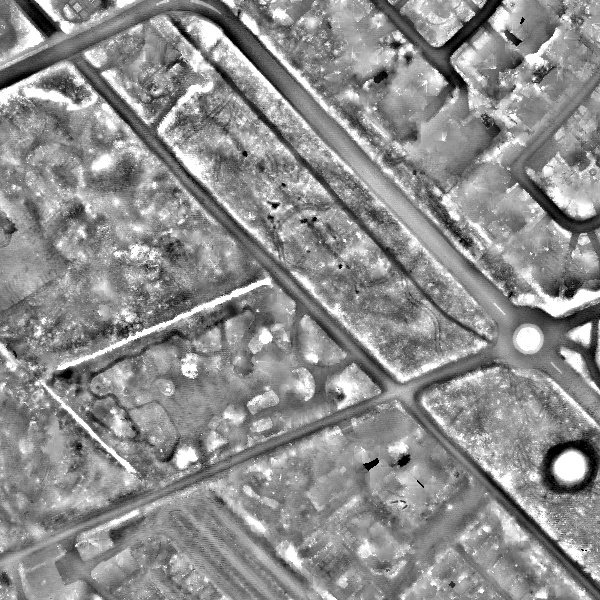
\includegraphics[width=0.75\textwidth]{lidarEx}
				\label{}
			\end{figure}
		\end{column}%
	\end{columns}

\end{frame}

\subsection{Archaeological Targets}
\begin{frame}
	\frametitle{Archaeological Targets: Barrows}
	\begin{columns}[T] % align columns
		\begin{column}{.48\textwidth}
			Barrows are mounds of raised earth or stone, over a burial placed in the middle - they are funerary monuments. They can be found all around Europe, and date from 2200BC to 1100BC. They are usually around 10 meters in diameters.
		\end{column}%
		\hfill%
		\begin{column}{.48\textwidth}

			\begin{figure}
				\centering
				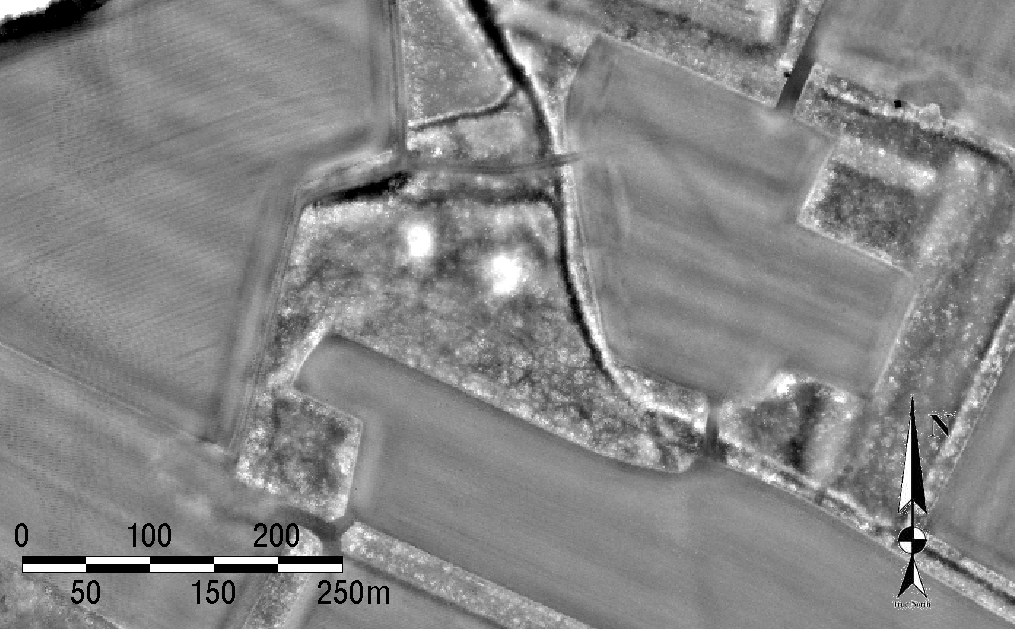
\includegraphics[width=\textwidth]{barrowsEx}
				\label{}
			\end{figure}
		\end{column}%
	\end{columns}
\end{frame}

\begin{frame}
	\frametitle{Archaeological Targets: Celtic Fields}
	\begin{columns}[T] % align columns
		\begin{column}{.48\textwidth}
			Celtic Fields are traces of ancient agricultural field systems. They are often found in North Western Europe. They are divided in rectangular cells of about $30 \times 30$m. \textbf{In our annotation system, each cell is an Celtic Field object, not the entire field}
		\end{column}%
		\hfill%
		\begin{column}{.48\textwidth}

			\begin{figure}
				\centering
				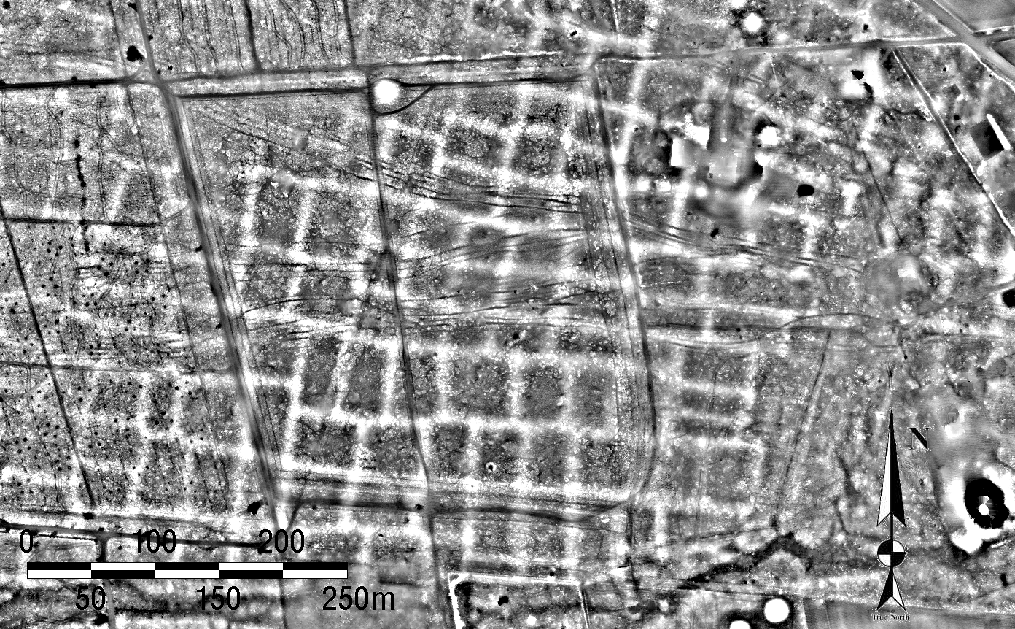
\includegraphics[width=\textwidth]{cfieldsEx}
				\label{}
			\end{figure}
		\end{column}%
	\end{columns}

\end{frame}

\begin{frame}
	\frametitle{Archaeological Targets: Charcoal Kilns}
	\begin{columns}[T] % align columns
		\begin{column}{.48\textwidth}
			Charcoal Kilns are circular structure used for coal production. They can be found all around Europe, and mostly around forests. Each charcoal kiln is about 5-10 meter in diameter, and are often found in groups.
		\end{column}%
		\hfill%
		\begin{column}{.48\textwidth}

			\begin{figure}
				\centering
				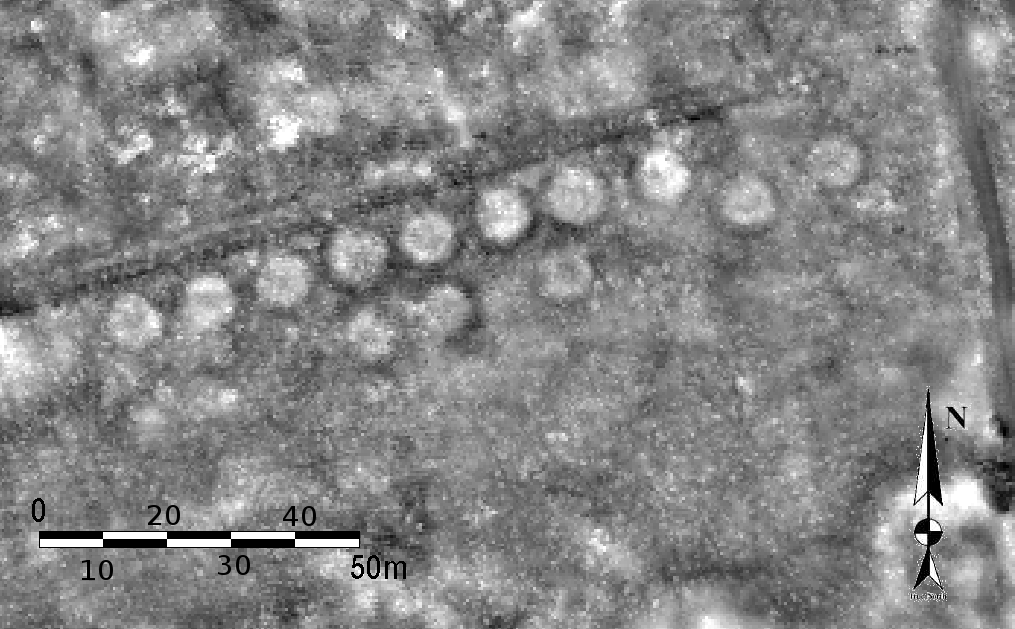
\includegraphics[width=\textwidth]{cKilnsEx}
				\label{}
			\end{figure}
		\end{column}%
	\end{columns}


\end{frame}

\subsection{Metrics}
\begin{frame}
	\frametitle{Precision, recall and F1-Score}

	\begin{columns}[T] % align columns
		\begin{column}{.48\textwidth}
			\begin{itemize}
				\item Precision is the percentage of correct predictions (True Positives) over all the predictions (True Positives and False Positives)
				\item Recall is the percentage of correct precision over all correct elements (True Positive and False Negatives)
				\item The $F_1$ Score is the harmonic mean of Precision and Recall
					\begin{equation}
						F_1 = 2 \times \frac{\text{precision} \times \text{recall}}{\text{precision} + \text{recall}}
					\end{equation}
			\end{itemize}
		\end{column}%
		\hfill%
		\begin{column}{.48\textwidth}
			\begin{figure}
				\centering
				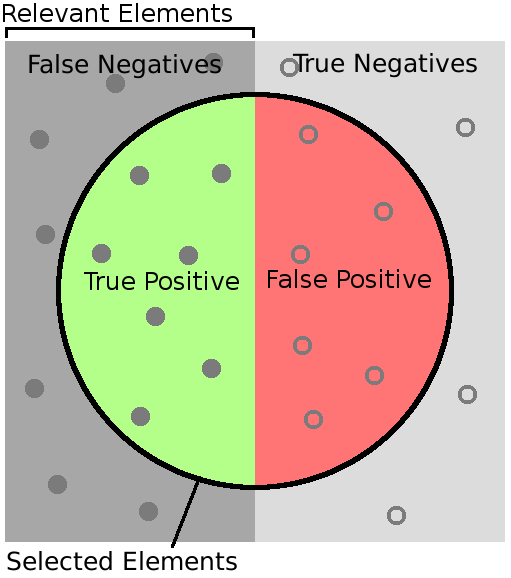
\includegraphics[width=0.6\textwidth]{precisionRecall}
				\caption[]{Precision and Recall}
				\label{}
			\end{figure}
		\end{column}%
	\end{columns}
\end{frame}

\begin{frame}
	\frametitle{IoU(s)}
	\begin{columns}[T]
		\begin{column}{.48\textwidth}
		\begin{itemize}
			\item Intersection over Union (IoU) is a measure of the quality of a bounding box
			\item It is computed by dividing the intersection of the predicted bBox and the ground truth bBox by the union of those two bBox
			\item There is ongoing research toward a better IoU: see GIoU, CIoU, DIoU...
		\end{itemize}
		\end{column}
		\hfill
		\begin{column}{.48\textwidth}
		\begin{figure}
		  \centering
			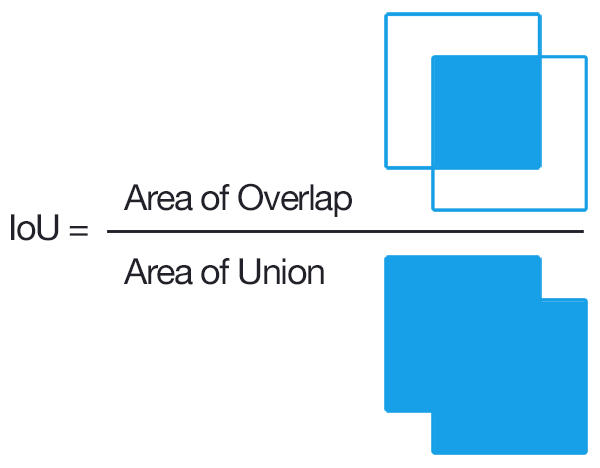
\includegraphics[width=0.5\textwidth]{iou}
		  \label{}
			\begin{equation}
				IoU = \frac{\text{area}(BBox_{truth} \cap BBox_{pred})}{\text{area}(BBox_{truth} \cup BBox_{pred})}
			\end{equation}
		\end{figure}
		\end{column}
		\end{columns}
\end{frame}

\begin{frame}
	\frametitle{mAP}
		The mean Average Precision (mAP) is a popular metric for object detector as is computed as follows:
		\begin{itemize}
			\item Draw a list of all the predictions made by the model, and rank them by predicted confidence level
			\item Compute the area under this curve: $AP = \int_0^1 p(r) dr$, with $p(r)$ being the precision of the model given a recall value
			\item the mAP\@50 is simply the AP average over all classes for IoU that are over 0.5
		\end{itemize}
\end{frame}

\section{Challenges}
\begin{frame}
	\begin{columns}[T] % align columns
		\begin{column}{.48\textwidth}
		\begin{itemize}
			\item Occlusion is a common issue in object detection
			\item In Aerial Remote Sensing, Vegetation might also pose a problem, with trees covering the ground 
			\item Large Earthworks, such as Barrows, might not be recognized as of Archaeological importance, and be partially destroyed to make way for new constructions
		\end{itemize}
		\end{column}
			\hfill
		\begin{column}{.48\textwidth}
		\begin{itemize}
			\item Remote Sensing Surveys are \textbf{large}, both in resolution and in amount of terrain covered
			\item This means that downscaling, usually done by detection frameworks destroys precious information !
			\item In Archaeology, this also means that manual verification, by way of prospection or otherwise is very difficult as it involves hundreds if not thousands of objects, separated by kilometers !
		\end{itemize}
		\end{column}
	\end{columns}

\end{frame}


	\section{State of the Art}
	\subsection{Archaeological Target Detection in Geophysical Data}

	\begin{frame}
		\frametitle{Learning To Look At LiDAR}
		This paper by Verschoof-van der Vaart and Lambers\cite{wouter2019} present both a new dataset and applies a Deep Learning based object detection framework.
	\begin{columns}[T] % align columns
		\begin{column}{.48\textwidth}
		\begin{itemize}
			\item Same 3 classes as discussed previously: barrows, Celtic fields and charcoal kilns 
			\item Dataset comprised of LiDAR surveys from central Netherlands, about 2350 $km^2$ covered
		\end{itemize}
		\end{column}
			\hfill
		\begin{column}{.48\textwidth}
		\begin{itemize}
			\item The model is a tweaked version of Faster-RCNN\cite{FasterRCNN} 
			\item Two different backbones were experimented with: ResNet50\cite{resNet} and VGG16\cite{vgg}
			\item Encouraging results were obtained, but charcoal kilns were not detected
		\end{itemize}
		\end{column}
	\end{columns}

	\end{frame}

	\begin{frame}
		\frametitle{Combining Deep Learning and Location-Based Ranking for Large-Scale Archaeological Prospection of LiDAR Data from The Netherlands}
		This paper by  Lambers, Verschoof-van der Vaart and Bourgeois\cite{verschoofAl2020} improves on previous results by combining an object detector and domain knowledge 
	\begin{columns}[T] % align columns
		\begin{column}{.48\textwidth}
		\begin{itemize}
			\item Same surveys as before 
			\item WODAN 2.0 now also contains negatives examples 
		\end{itemize}
		\end{column}
			\hfill
		\begin{column}{.48\textwidth}
		\begin{itemize}
			\item The model is a tweaked version of Faster-RCNN\cite{FasterRCNN}
			\item Domain Knowledge in the form of Location Based Ranking was used 
			\item This version obtained even better performance than WODAN 1.0 and was able to detect charcoal kilns  
		\end{itemize}
		\end{column}
	\end{columns}
	\end{frame}

	\subsection{Target Detection in Satellite Imagery}
	\begin{frame}
		\frametitle{Automated Detections in Satellite Imagery}
		A lot of work has been done in the past years to improve detections of objects in satellite imagery. Since they share many of the challenges we face in automated LiDAR detection, their solutions might apply to our case:
		\begin{itemize}
			\item You Only Look Twice, Van Etten\cite{yolt}
			\item A Simple and Efficient Network for small Target Detection, Ju \texit{et al.}\cite{sen}
			\item Object Detection in Remote Sensing Images Based on Improved Bounding Box Regression and Multilevel Features Fusion, Qian \textit{et al.} \cite{qianAl}
			\item A Single Shot Framework with Multi-Scale Feature Fusion for Geospatial Object Detection\cite{zhuang2019}
		\end{itemize}
		A (much more) comprehensive review is available as its own document. 
	\end{frame}

	\subsection{YOLOv4}
	\begin{frame}
		\frametitle{General Principle} 
		YOLO\cite{yolov1} is one of the fastest object detector on the market, and is widely considered as the SoTA for object detections. Its basic operating principle is as follows:
		\begin{itemize}
			\item Does one pass on the image $\rightarrow$ You Only Look Once
			\item Divide the input image into $S \times S$ grid, and predicts $B$ bounding boxes and confidence score for each cell
			\item Predicts an $S \times S \times (B \times 5 + C)$ tensor  
			\item Essentially rephrase the detection and classification problem into a regression one
			\item Blazing fast and accurate!
		\end{itemize}
	\end{frame}

	\begin{frame}
		\frametitle{Latest Improvements: Architecture} 

		YOLOv4\cite{yolov4} tried a wide range of architecture modules: 
		\begin{itemize}
			\item Attention Modules (SAM)\cite{sam}
			\item Receptive Fields Improvements (SPP)\cite{spp}
			\item Feature Fusion: Cross-stage partial Connections, multi-input weighted residual connections
			\item Path Aggregation (PAN)\cite{pan}
			\item Novel Losses: Mish\cite{mish} and Swish\cite{swish}
			\item \textbf{Novel IoUs}: DIoU\cite{diou}, CIoU\cite{diou}, GIoU\cite{giou}...  
			\item And much more ! 
		\end{itemize}
	\end{frame}

	\begin{frame}
		\frametitle{Latest Improvements: Training}
		YOLOv4 also heavily experimented with training regimes enhancements, the most notable being:
		\begin{itemize}
			\item Self Adversarial Training
			\item \textbf{Mosaic Data Augmentation}
			\item Cosine Annealing Scheduler
			\item Cross Mini-Batch Normalization
			\item And more...
		\end{itemize}
	\end{frame}

\section{Implementation}
\subsection{Dataset}
\begin{frame}
	\frametitle{Dataset details}
		\begin{column}{.48\textwidth}
			\begin{itemize}
				\item The original dataset from WODAN was constructed using LiDAR surveys from the Veluwe Region, Netherlands
				\item This data came in the form of a dozen TIFs, along with annotation in GIS form
			\end{itemize}
		\end{column}%
		\hfill%
		\begin{column}{.48\textwidth}
			\begin{itemize}
				\item For each object in the dataset, we centered an segment of a fixed size, with an added jitter of $\pm$ 100 pixels
				\item Bounding boxes are encoded in the COCO format: $(x, y, width, height)$
				\item All in all, the datasets contained about 7500 images. Some images contained multiples examples of objects, some none.
			\end{itemize}
		\end{column}%
\end{frame}


\begin{frame}
	\frametitle{Versions and annotations}
	\begin{itemize}
		\item The dataset went through multiple versions, testing how resolution and negative examples might affect accuracy
			\begin{itemize}
				\item V1: $1000 \times 1000$ pixels image, reuse of objects 
				\item V2: $1000 \times 1000$ pixels image, no reuse of objects $\rightarrow$ loss of performance 
				\item V3: $500 \times 500$ pixels image, reuse of objects
				\item V4: $1000 \times 1000$ pixels image, reuse of objects, addition of 1000 image in random coordinates and Negative Examples
			\end{itemize}
		\item V4: version gave the best results 
	\end{itemize}
\end{frame}

\subsection{Model Architecture and Training}
\begin{frame}
	\frametitle{Model Architecture and Training}
	Our model is based upon YOLOv4, and we experimented with the following modules:
	\begin{column}{.48\textwidth}
		Architectural:
	\begin{itemize}
		\item IoUs: GIoU, DIoU, CIoU
		\item Non Maximum Supressions: DNMS, NMS
		\item Different non linear units: Mish, Swish, SeLU, ReLU...
		\item Receptive Fields : Dilated Convolutions Modules, SPP...
		\item Various Input Pixel Size
		\item Optimized \textit{vs} unoptimized anchors 
	\end{itemize}
	\end{column}
	\hfill%
	\begin{column}{.48\textwidth}
	Training:
	\begin{itemize}
		\item Mosaic Data Augmentation
		\item Different datasets
		\item Different losses 
		\item Learning rate tweaks 
	\end{itemize}
	\end{column}
\end{frame}

\subsection{Best Model}
\begin{frame}
The best Model uses the following:
\begin{itemize}
	\item Distance Non Maximum Supression
	\item GIoU
	\item CV2 Data Augmentation
	\item Mosaic Data Augmentation
	\item $516 \times 516$ pixels input size
\end{itemize}
\end{frame}
\section{Results}
\subsection{Metrics}
\begin{frame}
	\frametitle{Per Class Accuracy}
	\begin{table}[h]
		\centering
		\begin{tabular}{@{}llll@{}}
			\toprule
				      & Kilns           & Barrows         & Celtic Field    \\ \midrule
				      Faster-RCNN\cite{wouter2019}& ---             & 55\%             & 58\%             \\
				      WODAN 2.0\cite{verschoofAl2020}& 12\% & 73\%             & 66\%             \\
				      Vanilla YOLOv4                & 63.04\%          & 77.04\%          & 85.73\%          \\
				      Our Model & \textbf{82.37\%} & \textbf{80.50\%} & \textbf{95.92\%} \\ \bottomrule
		\end{tabular}
				      \label{tab:resClasses}
	\end{table}
\end{frame}

\begin{frame}
	\frametitle{General Performance Metrics}
	\begin{table}[h]
		\centering
		\begin{tabular}{@{}lllllll@{}}
			\toprule
				      & Precision     & Recall        & F1-Score      & Av. IOU    & map@50         \\ \midrule
				      Faster-RCNN\cite{wouter2019} & ---           & ---           & 0.63          & ---            & ---            \\
				      WODAN 2.0\cite{verschoofAl2020} & ---           & ---           & 0.37 & ---            & ---            \\
				      Vanilla YOLOv4                & 0.58          & 0.84          & 0.69          & 45.75\%          & 75.27\%          \\
				      Our Model  & \textbf{0.64} & \textbf{0.93} & \textbf{0.76} & \textbf{57.48\%} & \textbf{86.27\%} \\ \bottomrule
		\end{tabular}
	\end{table}
\end{frame}

\begin{frame}
	\frametitle{Confusion Matrix}
	A confusion matrix shows which classes are being confused for which other classes. A perfect model would mean a diagonal matrix.
	\begin{table}[H]
	\centering
	\begin{tabular}{ll|ccc}
		&              & \multicolumn{1}{l}{} & \multicolumn{1}{l}{Predictions} & \multicolumn{1}{l}{} \\ \cline{3-5} 
								      &              & Kiln                 & Celtic Field                    & Barrow               \\ \hline
								      \multicolumn{1}{l|}{}      & Kiln         & 0.93           & 0.01                      & 0.05           \\
								      \multicolumn{1}{l|}{Truth} & Celtic Field & 0.01 & 0.95    & 0.06 \\
								      \multicolumn{1}{l|}{}      & Barrow       & 0.02 & 0.19 & 0.73
	\end{tabular}
	\label{tab:confMatYOLO}
\end{table}


\end{frame}
\begin{frame}
	\frametitle{Analysis}
	\begin{itemize}
		\item An optimised YOLO significantly outperforms a Vanilla YOLOv4 on this task 
			\begin{itemize}
				\item Tweaking and experimenting is worth it
			\end{itemize}
		\item Slight class confusion between Barrow and Celtic Fields
			\begin{itemize}
				\item Might be an indicator of low amount of examples 
			\end{itemize}
		\item Our model also outperform the State of the Art 
		\item My personal PoV: using the latest object detection frameworks and tweaking it is the key to best performance, rather than domain knowledge
			\begin{itemize}
				\item But using both would be even better !
			\end{itemize}
	\end{itemize}
\end{frame}

\subsection{Integration into a GIS: QGIS and CSV}
\begin{frame}
	\frametitle{Integration}
	\begin{itemize}
		\item We are also able to integrate the detection results into a Geographical Information Software for easier analysis
		\item We simply collect all detection results on all the images and their coordinates and confidence
		\item After a transformation from image coordinates to a specific coordinates reference system, the detection are stored in a CSV database
		\item Import to QGIS\cite{QGIS_software} is then done in a few clicks
		\item Post detection analysis is way easier using dedicated software ! 
	\end{itemize}
\end{frame}

\subsection{The Good Stuff: Detection Examples !}
{
	\usebackgroundtemplate{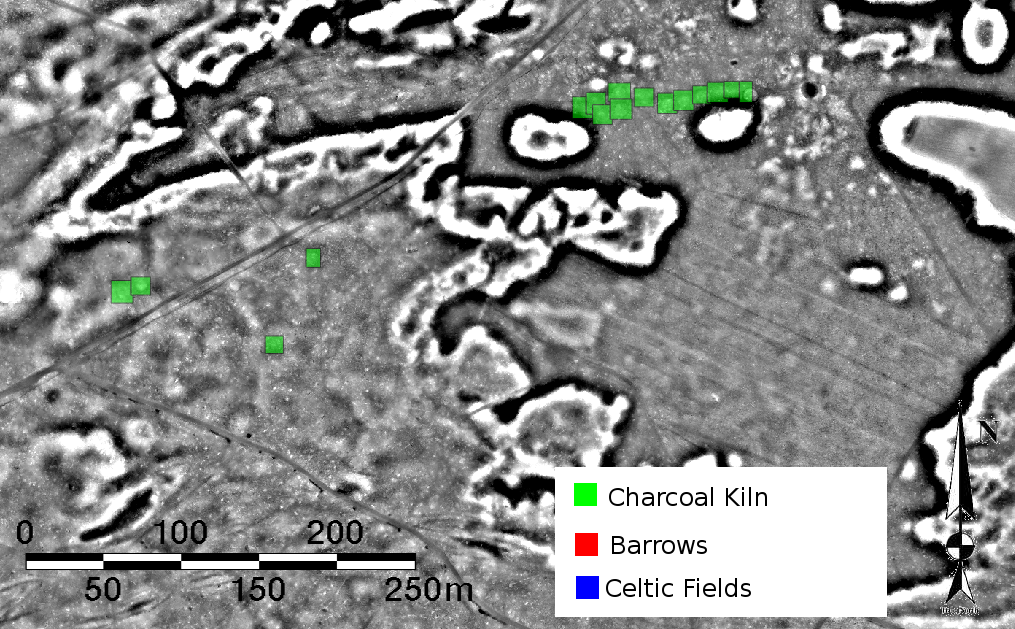
\includegraphics[height=\paperheight,width=\paperwidth]{detectionsExample1}}
	\begin{frame}[plain]
	\end{frame}
}
{
	\usebackgroundtemplate{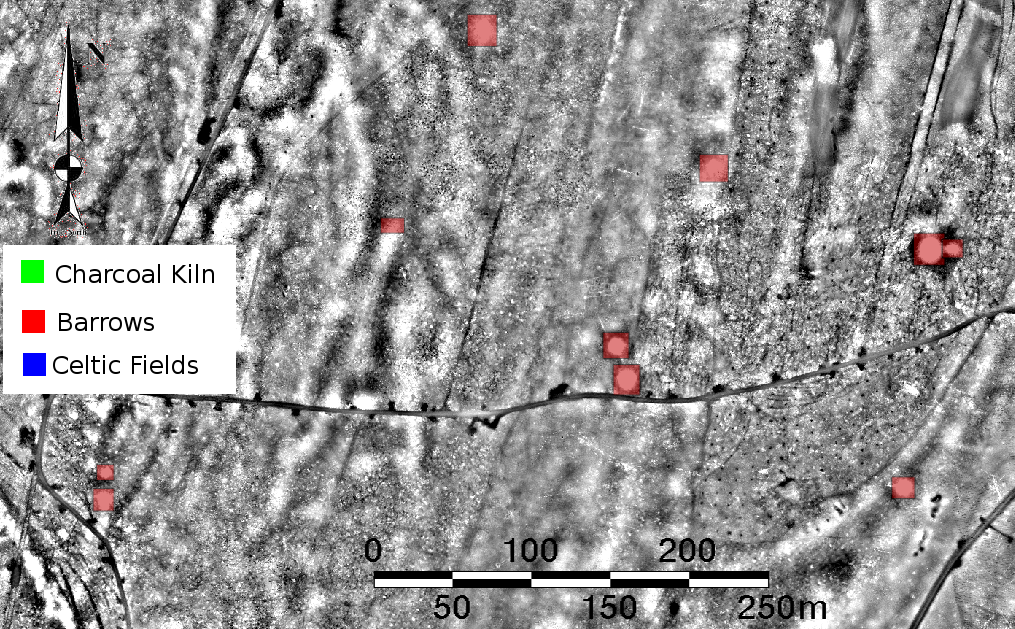
\includegraphics[height=\paperheight,width=\paperwidth]{detectionsExample2}}
	\begin{frame}[plain]
	\end{frame}
}
{
	\usebackgroundtemplate{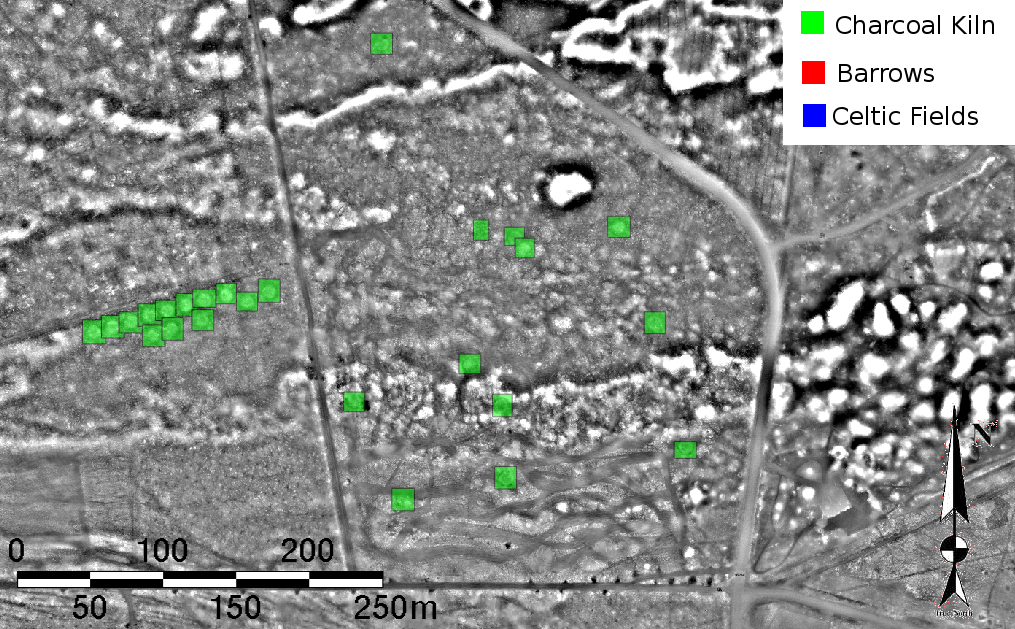
\includegraphics[height=\paperheight,width=\paperwidth]{detectionsExample3}}
	\begin{frame}[plain]
	\end{frame}
}

\section{Conclusions}
\subsection{Discussion}
\begin{frame}
	\frametitle{Discussion}

	\begin{columns}[T] % align columns
		\begin{column}{.48\textwidth}
		\begin{itemize}
			\item Our system is accurate on all classes, and fast ! About 5 minutes for all 2350 $km^2$
			\item A modified and finetuned model is able to outperform models with added domain information
			\item Occlusion and confusion is still an issue $\rightarrow$
		\end{itemize}
		\end{column}
		\begin{column}{.48\textwidth}
		
		\begin{figure}
		  \centering
			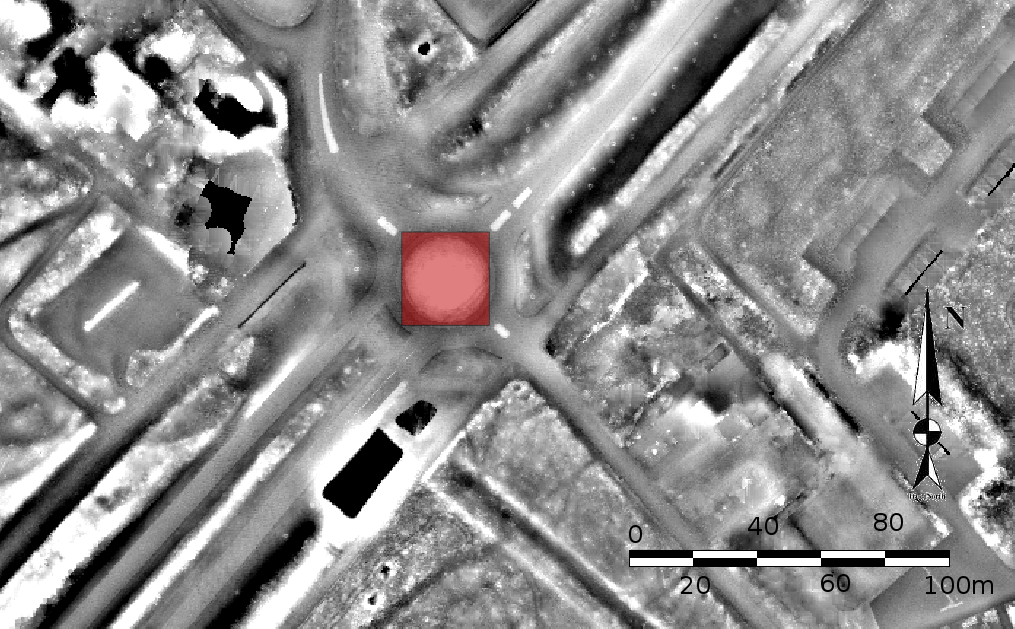
\includegraphics[width=0.9\textwidth]{wrongBarrow}
			\caption{Confusion between a barrow and a roundabount}
		  \label{}
		\end{figure}
		\end{column}
		\end{columns}
\end{frame}

\subsection{Further Improvements}
\begin{frame}
	\frametitle{Further Improvements and what's next}
	\begin{columns}[] % align columns
		\begin{column}{.48\textwidth}
	\begin{itemize}
		\item Semantic Segmentation with a SoTA model like Fast-FCN or Gated-SCNN
		\item Multi Data Inference: Use of multiple type of input data, like a combination of satellite imagery and LiDAR survey 
		\item Integration of domain knowledge, as in WODAN2.0\cite{verschoofAl2020} 
		\item Redaction of an article to present those results ! 
	\end{itemize}
	\end{column}
			\hfill
		\begin{column}{.48\textwidth}
		\begin{figure}
		  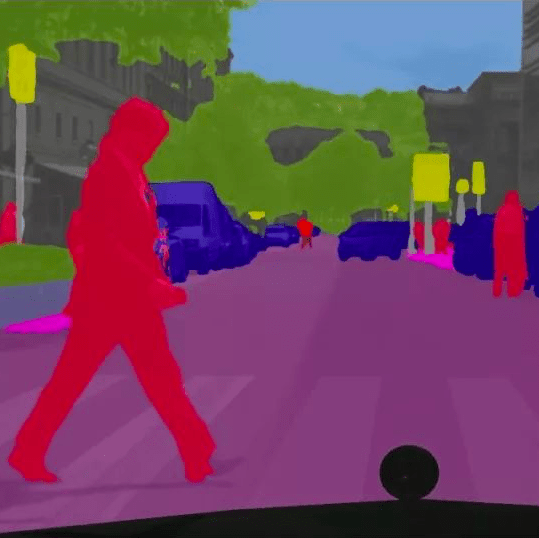
\includegraphics[width=0.8\textwidth]{semseg}
			\caption{Semantic Segmentation}
		\end{figure}
	\end{column}
	\end{columns}

\end{frame}

\begin{frame}
	\frametitle{Question Time !}
	\centering
	\Huge{Thank you for your attention\\
	Any questions ?}
\end{frame}

\begin{frame}[allowframebreaks]
	\printbibliography[heading=bibintoc]
\end{frame}
\end{document}
